\documentclass[a4paper,11pt,notitlepage,fullpage]{article}
%\documentclass{report}

\usepackage{fullpage}
\usepackage[utf8]{inputenc}
%\usepackage[ngerman]{babel}
%\usepackage[english]{babel}
\usepackage{amsmath}
\usepackage{amssymb}
\usepackage{latexsym}
\usepackage{mathtools}
\usepackage{listings}
\usepackage{bbm}
%\usepackage{algorithm}
%\usepackage{algpseudocode}
\usepackage{graphicx}
\usepackage{booktabs}
\usepackage{hhline}
\usepackage{amsthm}
\usepackage{cite}
\usepackage{wrapfig}
\usepackage{hyperref}
\usepackage{titling}
\usepackage{color}

\setlength{\droptitle}{-60pt}

\newcommand{\R}{\mathbb R}
\newcommand{\p}{\mathbb P}
\newcommand{\pp}[1]{\mathbb P\left[#1\right]}
\newcommand{\E}{\mathbb E}
\newcommand{\Ee}[1]{\mathbb E\left[#1\right]}
\newcommand{\V}{\mathbb V}
\newcommand{\Vv}[1]{\mathbb V\left[#1\right]}
\newcommand{\Cov}[1]{\mathbb Cov\left[#1\right]}
\newcommand{\F}{\mathcal{F}}
\newcommand{\ind}{\mathbbm{1}}
\newcommand{\indd}[1]{\mathbbm{1}_{#1}}
\newcommand{\norm}[2]{\left|\left|{#1}\right|\right|_{#2}}

\begin{document}
\author{Florian Bogner \& Alexander Palmrich}
\title{Stochastische Prozesse - Übung 5}
\maketitle

\begin{enumerate}
\setcounter{enumi}{20}

%21
\item Sei 
\begin{align*}
f(t) &:= W(t) \indd{[0,1)}(t)\\
f_n(t) &:= \sum_{j=0}^{n-1} W(\frac{j}{n}) \indd{[\frac{j}{n}, \frac{j+1}{n})}(t)\\
Y &:= \frac{W(1)^2-1}{2}
\end{align*}

\begin{figure}[h!]
\centering
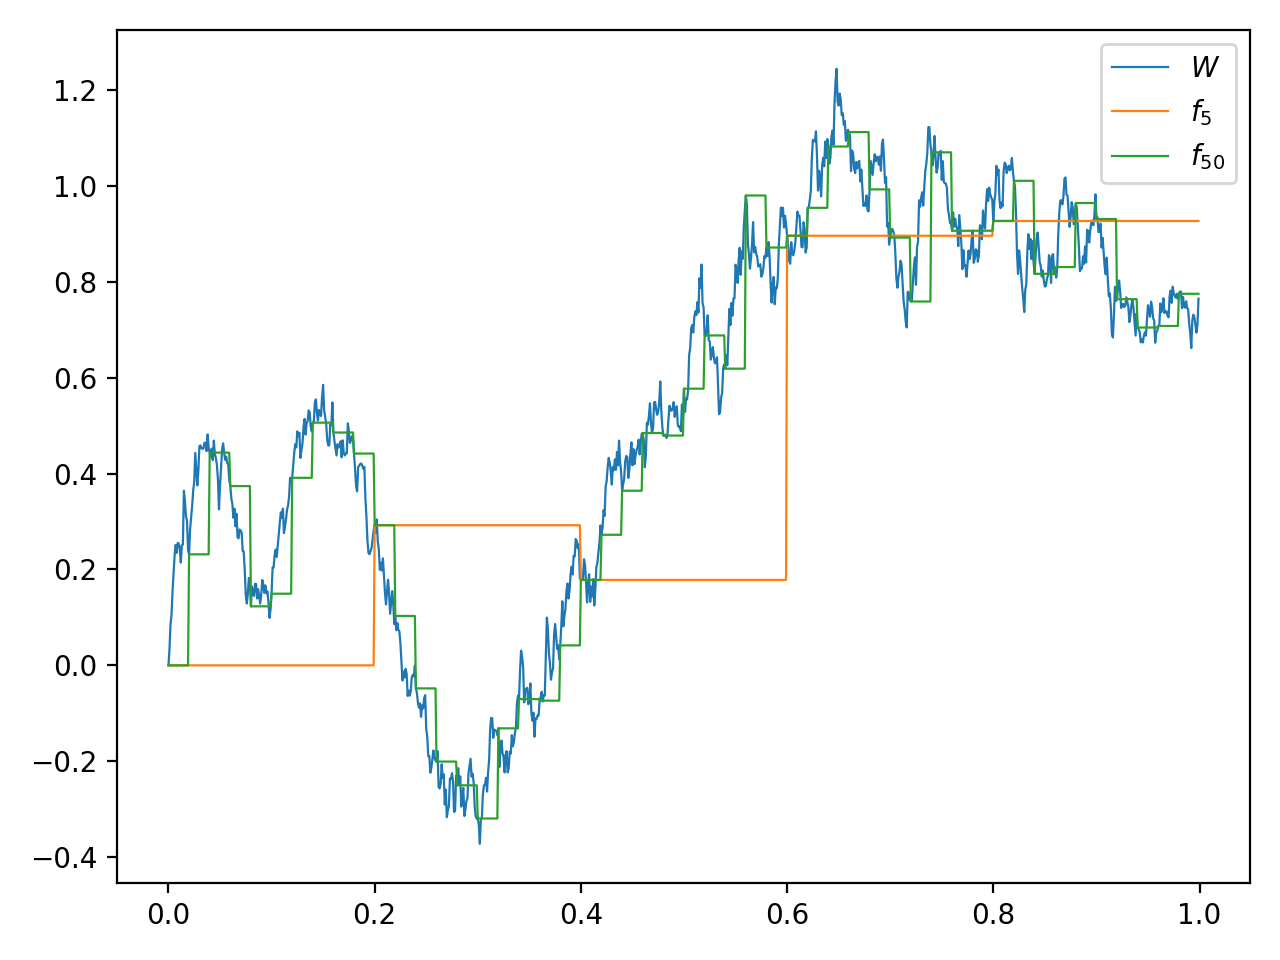
\includegraphics[width=0.9\textwidth]{gfx/21_fig.png}
\caption{Ein typischer Pfad von $f$ und $f_n$}
\end{figure}

\begin{enumerate}
%a
\item $M^2$-Fehler der Approximation von $f$ bestimmen.
\begin{align*}
\norm{f_n-f}{M^2} &= \norm{\sum_{j=0}^{n-1} \left(W(\frac{j}{n})-W(t)\right) \indd{[\frac{j}{n}, \frac{j+1}{n})}(t)}{M^2}\\
&= \Ee{\int \sum_{j=0}^{n-1} \left(W(\frac{j}{n})-W(t)\right)^2 \indd{[\frac{j}{n}, \frac{j+1}{n})}(t) dt}\\
&= \int \Ee{\sum_{j=0}^{n-1} \left(W(\frac{j}{n})-W(t)\right)^2 \indd{[\frac{j}{n}, \frac{j+1}{n})}(t) } dt &\text{(Fubini-Tonelli)}\\
&= \int \sum_{j=0}^{n-1} \Ee{\left(W(\frac{j}{n})-W(t)\right)^2} \indd{[\frac{j}{n}, \frac{j+1}{n})}(t)  dt\\
&= \int \sum_{j=0}^{n-1} \left(t-\frac{j}{n}\right) \indd{[\frac{j}{n}, \frac{j+1}{n})}(t)  dt & \text{($W$ neu gestartet)}\\
&=  \sum_{j=0}^{n-1} \int\left(t-\frac{j}{n}\right) \indd{[\frac{j}{n}, \frac{j+1}{n})}(t)  dt \\
&=  \sum_{j=0}^{n-1} \frac{1}{2n^2} & \text{($\int$ = halbes Quadrat der Länge $\frac{1}{n}$)}\\
&= \frac{1}{2n}
\end{align*}
Man beachte, dass mit Itô-Isometrie gilt
$$\frac{1}{2n} = \norm{f_n-f}{M^2} = \norm{I(f_n-f)}{L^2} = \norm{I(f_n)-I(f)}{L^2} = \norm{I(f_n)-Y}{L^2}$$

%b
\item $L^2$-Fehler der Approximation der Itô-Integrale, ohne Isometrie.
\begin{align*}
\norm{I(f_n)-Y}{L^2} = ?
\end{align*}
\end{enumerate}


%22
\item Sei
$$g_n(t) := \sum_{j=0}^{n-1} (W(\frac{j}{n}))^2 \indd{[\frac{j}{n}, \frac{j+1}{n})}(t)$$
\begin{enumerate}
%a
\item Varianz des Itô-Integrals ausrechnen.
\begin{align*}
\Vv{I(g_n)} &= \Ee{(I(g_n))^2}\\
&=\Ee{\int g_n^2 dt}\\
&= \int \Ee{g_n^2} dt\\
&= \int \Ee{\sum_{j=0}^{n-1} (W(\frac{j}{n}))^4 \indd{[\frac{j}{n}, \frac{j+1}{n})}(t)} dt\\
&= \int \sum_{j=0}^{n-1} \Ee{(W(\frac{j}{n}))^4} \indd{[\frac{j}{n}, \frac{j+1}{n})}(t) dt\\
&= \int \sum_{j=0}^{n-1} 3(\frac{j}{n})^4 \indd{[\frac{j}{n}, \frac{j+1}{n})}(t) dt &\text{(viertes Moment Normalverteilung)}\\
&= \sum_{j=0}^{n-1} 3(\frac{j}{n})^4 \int \indd{[\frac{j}{n}, \frac{j+1}{n})}(t) dt\\
&= \sum_{j=0}^{n-1} 3(\frac{j}{n})^4 \frac{1}{n} &(*)\\
&= \frac{3}{n^5} \sum_{j=0}^{n-1} j^4 \\
\end{align*}
In der Darstellung $(*)$ steht eine Riemannsumme zum Integral $\int_0^1 3x^4 dx$ mit äquidistanten Stützstellen $x_j = \frac{j}{n} \Rightarrow \Delta x = \frac{1}{n}$, womit diese Summe für $n\rightarrow \infty$ gegen $\left. \frac{3}{5}x^5\right|_0^1 = \frac{3}{5}$ geht.

%b
\item Summen über eine feste Potenz natürlicher Zahlen: Nach wem sind Formeln benannt, die sowas anders darstellen?

\begin{figure}[h!]
\centering
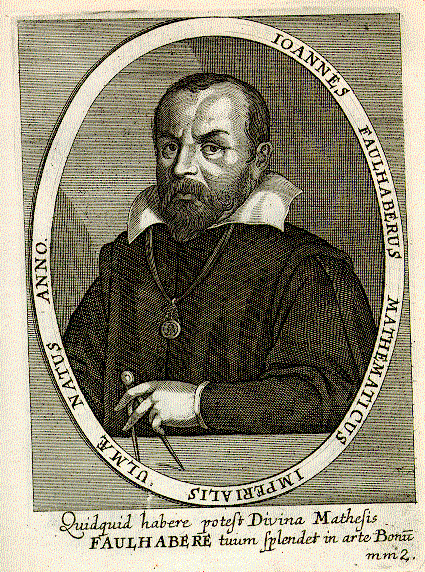
\includegraphics[width=0.9\textwidth]{gfx/Ioannes-Faulhaberus-Mathematicus-Imperialis-Ulmae-Natus.png}
\caption{Johannes Faulhaber}
\end{figure}

\textsc{Johannes Faulhaber}, der in der Spätrenaissance um 1600 herum gelebt hat, hat für $n=1..11$ konkrete Formeln aufgestellt.
Die allgemeine Familie der Identitäten
$$\sum_{j=0}^{n-1} j^k = \frac{1}{k+1}\sum_{j=0}^k \binom{k+1}{j} B_{j} n^{k+1-j} \in \text{\{Polynome in $n$ vom Grad $k+1$\}}$$
wobei $B_j$ die $j$-te Bernoulli-Zahl erster Art bezeichnet, ist daher nach Faulhaber benannt.
Fauhlaber war Mathematiker, Ingenieur, Festungsbaumeister (Basel und Frankfurt), Rechnenmeister, Numerologe, Alchemist, Astrologe, Erfinder, ein Freund Keplers.


Die \textsc{Erdős}-\textsc{Moser}-Gleichung hat die Gestalt
$$\sum_{j=0}^{m} j^k = (m+1)^k$$
und ordnet sich damit in die Familie ein. Eine bekannte Lösung lautet $1^1+2^1=3^1$, seit 70 Jahren hat man keine weitere Lösung gefunden, weiß aber dass $m>10^{1000000000}$ gelten müsste.

\textsc{Leo Moser}, Namensgeber obiger Gleichung, hat übrigens ein weiteres bisher ungelöstes, sehr elegantes Problem formuliert (Moser's worm problem):
\emph{Was ist eine Figur mit minimalem Flächeninhalt in der Ebene, so dass man jede Kurve der Länge $1$ einschreiben kann?}\\
Man weiß dass so eine Figur existieren muss (anders als beim Nadel-Umdreh-Problem beispielsweise), und seit 2017 auch dass ein Kreissektor, der $\frac{1}{6}$ des Einheitskreises ist, eine obere Schranke bildet.


Zurück zu den Summen: Wenn man $n\rightarrow \infty$ gehen lässt, konvergieren die Summen nicht mehr. Wenn wir aber negative Exponenten zulassen, oder gleich komplexe, dann landen wir schnell bei der Riemannschen Zeta-Funktion:
$$\zeta (z) := \sum_{n=1}^\infty \frac{1}{n^z}$$
Diese Funktion taucht vielerorts prominent auf und ist super wichtig, siehe Literatur.
\begin{align*}
\end{align*}
\end{enumerate}

%23
\item Markovkette mit vier Zuständen, Anfangsverteilung $\lambda = (0.5, 0.5, 0, 0)$ und der Übergangsmatrix
$$P=$$
\begin{enumerate}
%a
\item Wahrscheinlichkeiten von zwei konkreten Zustandsfolgen ausrechnen.
\begin{align*}
\end{align*}

%b
\item Kommunikationsklassen, Rekurrenz, Transienz.
\begin{align*}
\end{align*}

%c
\item Trefferzeit in $\{1, 4\}$.
\begin{align*}
\end{align*}

%d
\item Mittlere Trefferzeit wie oben aber bei Start in jeweiligen Zuständen ausrechnen.
\begin{align*}
\end{align*}

%e
\item Varianz der Trefferzeit wie oben bei Start in $3$ ausrechnen.
\begin{align*}
\end{align*}
\end{enumerate}

%24
\item Marovkette mit fünf Zuständen, Übergangswahrscheinlichkeiten siehe Graph.
\begin{enumerate}
%a
\item Wahrscheinlichkeiten von zwei konkreten Zustandsfolgen ausrechnen.
\begin{align*}
\end{align*}

%b
\item Kette irreduzibel?
\begin{align*}
\end{align*}

%c
\item Trefferzeiten für $0$ endlich mit welcher $\p$?
\begin{align*}
\end{align*}

%d
\item LGS für mittlere Trefferzeiten in $0$ aufstellen.
\begin{align*}
\end{align*}
\end{enumerate}

%25
\item Münzwurfspiel, $\pm 1$ Kapital je nach Kopf/Zahl. LGS lösen für die Wahrscheinlichkeiten, in endlicher Zeit in den Ruin zu kommen.


\end{enumerate}












\end{document}
